\chapter{Data}\label{chap:data}
\begin{chapabstract}

In this Chapter, we describe the dataset used for our study and procedures to select galaxy samples for further analysis.
In Section~\ref{sec:HerschelReferenceSurvey}, we introduce the Herschel Reference Survey Catalog \citep{Boselli2010}.
Here, we explain how they choose galaxies for the catalog and previous studies of them.
In Section~\ref{sec:gleamsurvey}, we introduce the GaLactic Extragalactic All-sky MWA survey, which we obtained the radio data for galaxy samples.
Section~\ref{sec:crossmatching} and~\ref{sec:reducegalaxysamples} show how to select samples from two catalogs introduced in the previous Section for $\qn$ analysis henceforth.
Section~\ref{sec:calculatingq} gives the definition of $\qn$ and the way to apply it for our samples.

\end{chapabstract}

\section{Herschel Reference Survey (HRS) Catalog}\label{sec:HerschelReferenceSurvey}
In this Section, we introduce the Herschel Reference Survey (HRS) catalog \citep{Boselli2010} from which we selected galaxy samples.
This survey is one of the Herschel guaranteed time key projects, and originally it was compiled for understanding dust properties and the interstellar medium in nearby galaxies.
The catalog is publicly available and contains 322 galaxies selected with three criteria as follows:

\begin{enumerate}
    \item Volume-limited:\\
        They choose galaxies whose distance from the earth is between $15$ and $25\,\mr{Mpc}$.
        This limitation reduces the distance uncertainty due to the galaxy peculiar motions and the selection effect due to the high-$z$ galaxies.
        The lower limit ($15\,\mr{Mpc}$) also helps us to observe sources within reasonable exposure time because very close galaxies us are extended, and we need too much time for the observation.
    \item $K$-band selection:\\
        They choose galaxies whose 2MASS $K$-band total magnitudes are brighter than $12\,\mr{mag}$ for star-forming and peculiar galaxies (Sa-Sd-Im-BCD), and $8.7\,\mr{mag}$ for quiescent galaxies (E, S0, S0a).
        If there are galaxies whose $K$-band magnitude darker than those values, their measurements are not regarded as accurate photometry because of not enough exposure time.
        The reason why they have selected quiescent galaxies with the more stringent $K$-band selection criteria is these galaxies are expected to have low dust contents, and it is difficult to detect within the reasonable exposure time.
    \item High galactic latitude:\\
        They choose galaxies whose galactic latitude is high enough to minimize the contamination from the galactic center ($b > +55^{\circ}$).
        Also, they select galaxies with the low galactic extinction ($A\msb{B} < 0.2$; \citealt{Schlegel1998}).
\end{enumerate}

The selected galaxies locate in the sky region between $10\msu{h}17\msu{m}< \mr{R.A.}(2000) < 14\msu{h}43\msu{m}$ and $-6^{\circ} < \mr{decl.} < 60^{\circ}$ (Figure~\ref{fig:Boselli2010_figure1}).
HRS galaxies span a wide range of the galaxy density environment from the center of the Virgo cluster to the isolated region.
As a definition, we can regard the HRS sample as an ideal one for studying the galaxy environment.

\begin{figure}[htbp]
	\centering
	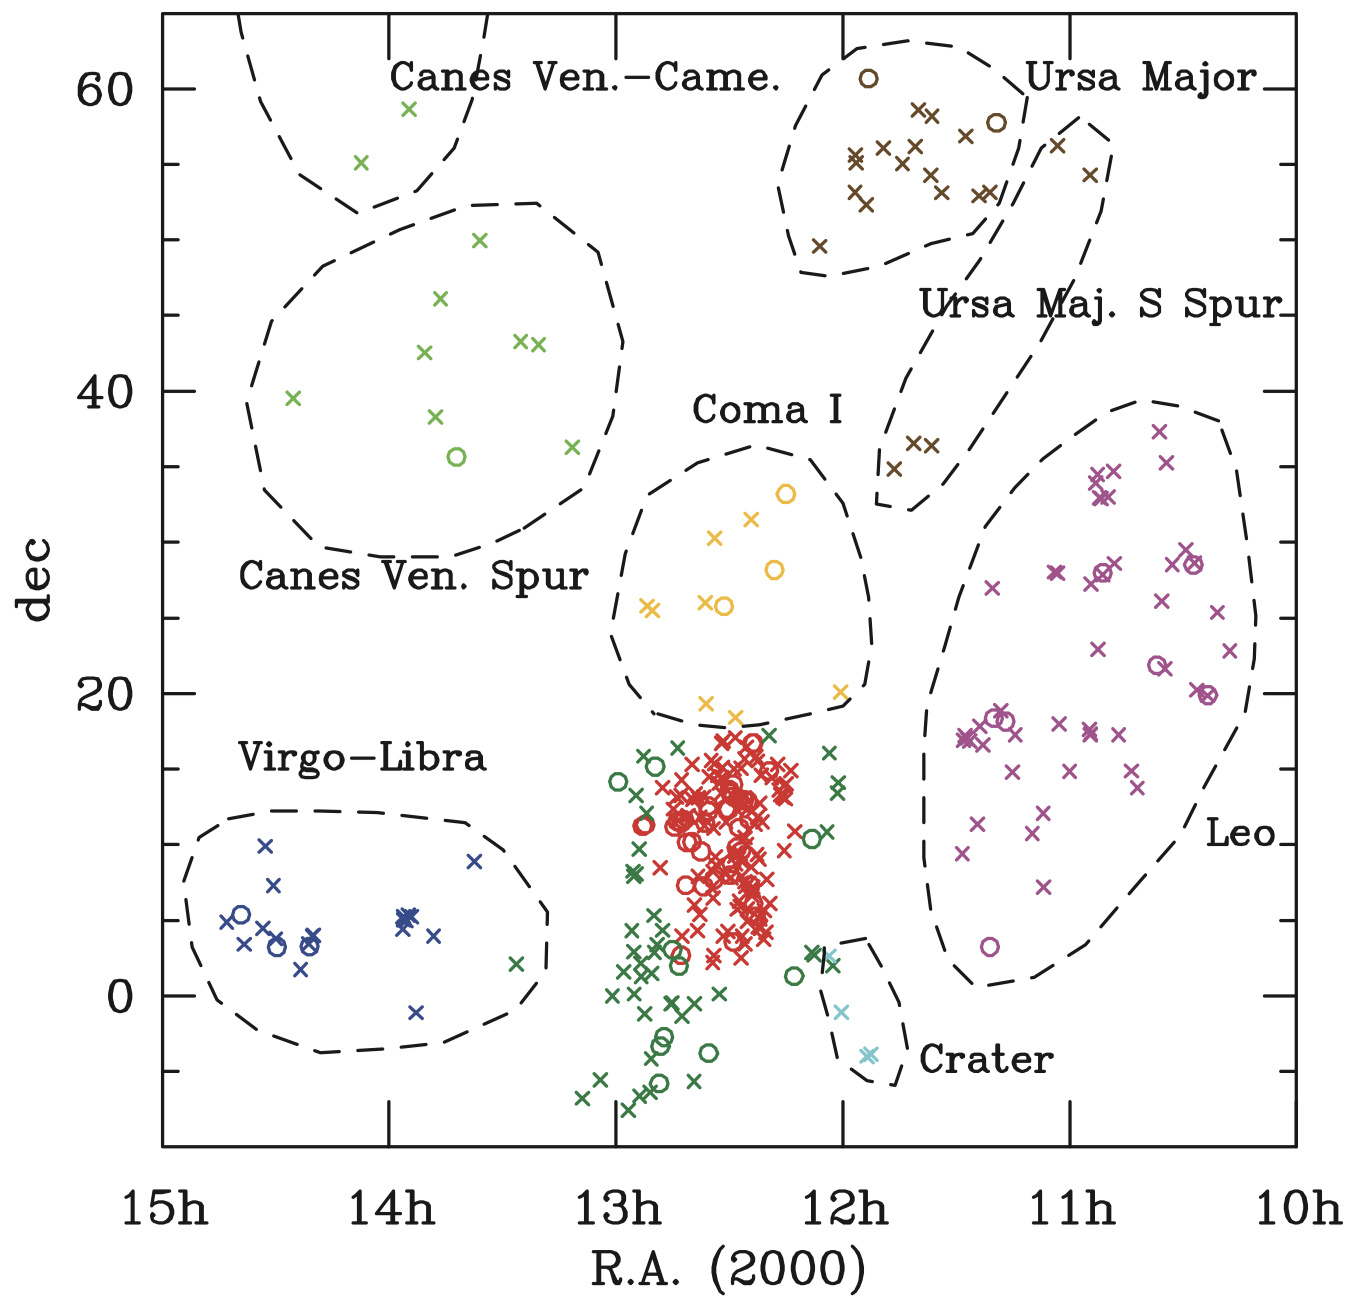
\includegraphics[width=.7\linewidth]{Chapter_3/Figures/Boselli2010_Figure1.png}
    \caption[The sky distribution of galaxies in HRS catalog]{\label{fig:Boselli2010_figure1}
        The sky distribution of the HRS galaxy sample.
        They show the early-type galaxies (E, S0, S0a) and late-type galaxies with circles and crosses, respectively.
        Dashed circles represents the different cloud regions. Each name of the cloud is shown close to each region.
        The red and dark green markers are Virgo galaxies (red: Virgo center, dark green: its outskirts).
        Reprint from \citealt{Boselli2010}, Figure~1.
    }
\end{figure}

In addition to a wide range of the environment, HRS galaxies distribute a wide range of galaxy morphology (Figure~\ref{fig:Boselli2010_figure2}).

\begin{figure}[htbp]
	\centering
	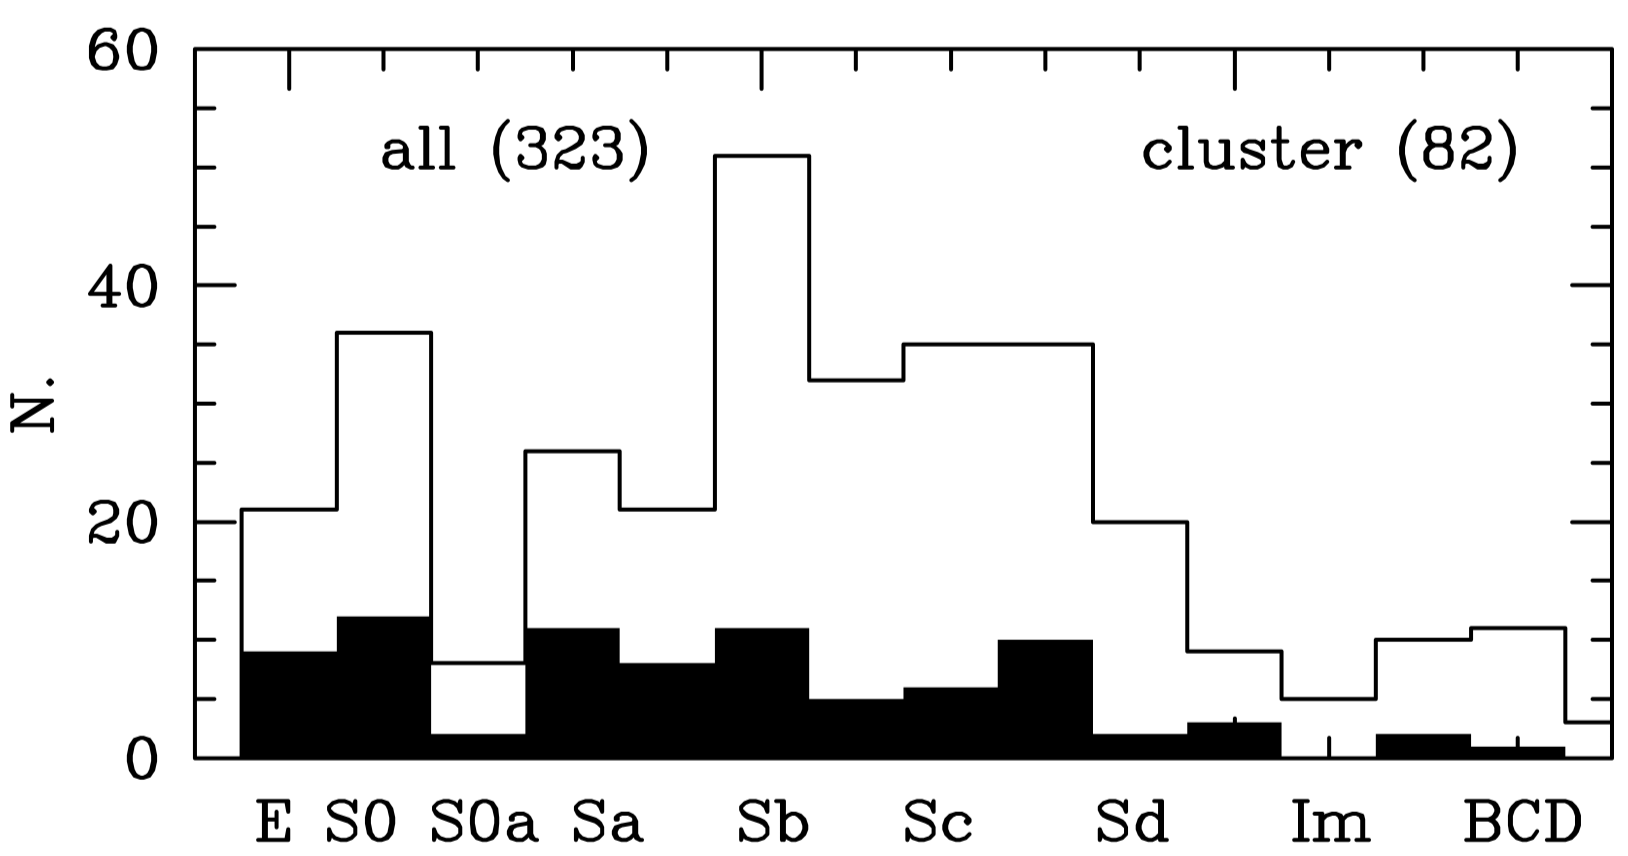
\includegraphics[width=.8\linewidth]{Chapter_3/Figures/Boselli2010_Figure2.png}
    \caption[The morphology distribution of HRS samples]{\label{fig:Boselli2010_figure2}
        The distribution in the morphology-type of HRS galaxies.
        The shaded histogram represents the distribution in it of only the cluster sample.
        Here, the cluster sample composed of HRS galaxies located in the Virgo A and B clouds.
        Reprint from \citealt{Boselli2010}, Figure~2.
    }
\end{figure}

Since HRS galaxies are supposed to be well-represented for the whole galaxy population located in the local Universe, investigating their physical properties is crucial to understand them.
After \citet{Boselli2010} published the HRS catalog, many studies investigating the physical properties for HRS galaxies have been done until now.
Here, we introduce some of the studies for the HRS sample.
\citet{Cortese2012} investigated their UV and optical properties using the Galaxy Evolution Explorer ({\it GALEX\/};~\citealt{Martin2005}) and SDSS-DR7 \citep{Abazajian2009}.
\citet{Boselli2014} studied their cold gas properties with $^{12}\mr{CO}\brp{1-0}$ observed by the Kitt Peak 12m radio telescope and obtained from the literature data.
They also investigate the \nh~gas obtained from The Arecibo Legacy Fast ALFA (ALFALFA;~\citealt{Giovanelli2005, Haynes2011}) survey.
\citet{Ciesla2014} executed the SED fitting for HRS galaxies with Code Investigating GALaxy Emission (CIGALE;~\citealt{Noll2009}).

Thanks to all of the previous research about the HRS sample, they are well-studied from the X-ray to the radio emission at $1500\MHz$.
However, the low-frequency around $100\MHz$ is not examined so far.
Since we would like to extend the wavelength range of the HRS sample to around $100\MHz$, in this study, we focus on a subsample of HRS galaxies whose counterpart is detected by the latest low-frequency survey (Section~\ref{sec:gleamsurvey}).



\section{The GaLactic Extragalactic All-sky MWA (GLEAM) Survey Catalog}\label{sec:gleamsurvey}

In this Section, we introduce the GaLactic Extragalactic All-sky MWA (GLEAM) survey \citep{Hurley-Walker2017a}, which we obtained the radio continuum data from.
This survey was operated by the Murchison Widefield Array (MWA) telescope in Western Australia \citep{Tingay2013a}.
It observed a whole southern sky and a northern sky up to $+30^{\circ}$ (24,831 $\mathrm{\deg}^2$;~Figure~\ref{fig:HurleyWalker2017_figure11}).
The catalog from this survey is publicly available and contains 307,455 detected radio sources with fluxes at 20 narrow bands between $72$ and $231\MHz$ (each band has $7.68\MHz$ bandwidth).

The observations of this survey were operated by the grouped five bands with $30.72\MHz$ bandwidth.
These grouped bands have the center at $87.7$, $118.4$, $154.2$, $185.0$, $215.7\MHz$, respectively.
Because of the orbcomm satellite interference, They did not observe at $134\mbox{--}139\MHz$.
The observation was executed sequentially as $112\,\mr{s}$ snapshots (each frequency was observed every $10\,\mr{minutes}$).
The sensitivity and angular resolution at $200\MHz$ are $\sim 7\,\mr{mJy}$ and $\sim 2\,\mr{arcmin}$ respectively.
The completeness of this survey at $200\MHz$ is $90\%$ at $\sim 170\mr{mJy}$.
Since this survey allows us to examine the low-frequency spectral energy distribution accurately with its 20 narrow bands, we adopt the radio source catalog for our study.

\begin{figure}[htbp]
	\centering
	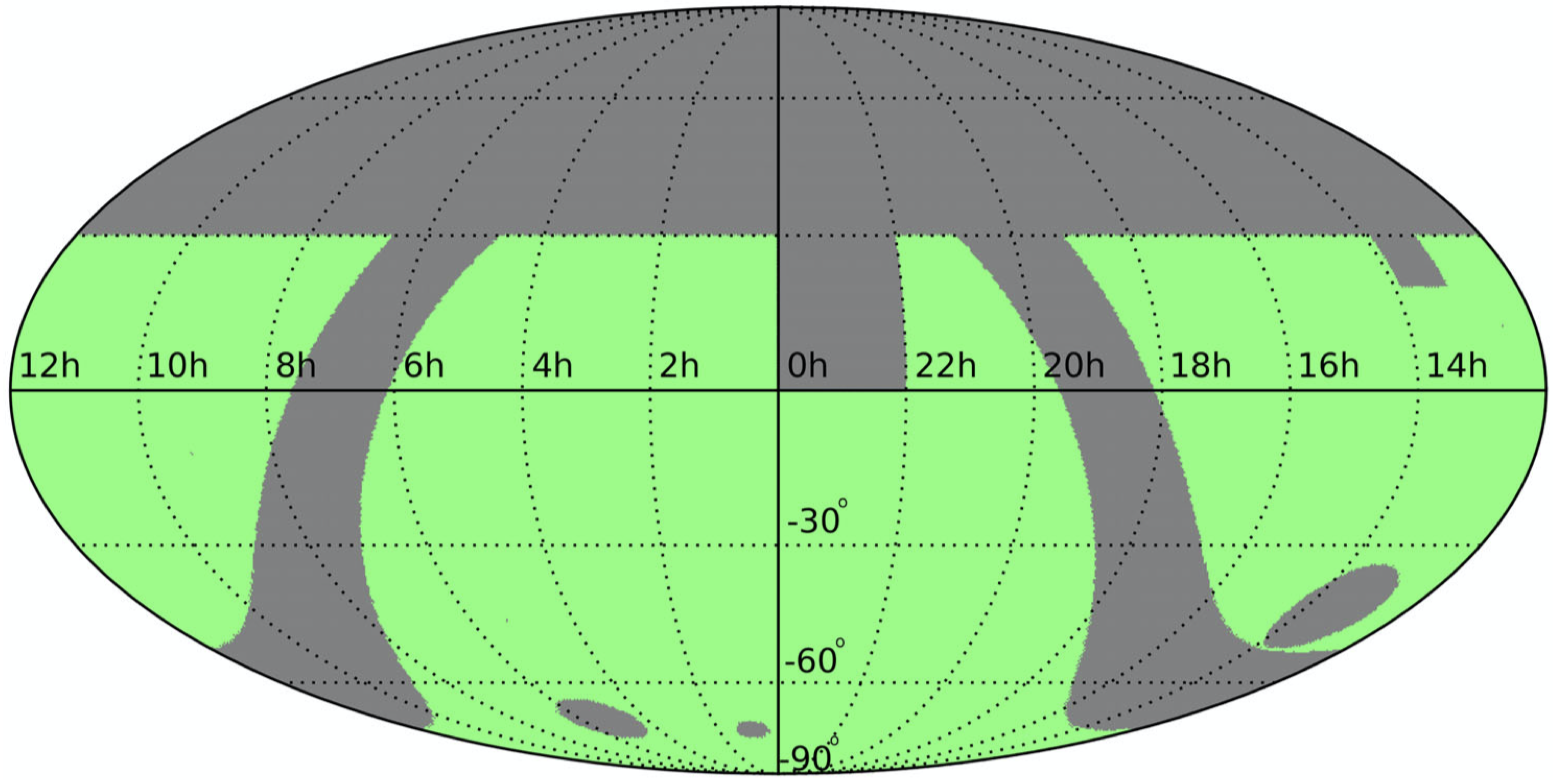
\includegraphics[width=.7\linewidth]{Chapter_3/Figures/HurleyWalker_Figure11.png}
    \caption[The observing area of the GLEAM survey]{\label{fig:HurleyWalker2017_figure11}
        The observed area by the GLEAM survey (green shaded region).
        \citet{Hurley-Walker2017a} exclude several regions intentionally to minimize the contamination:
        Galactic plane (Absolute Galactic latitude $<10^{\circ}$),
        Ionospherically distorted ($0^{\circ} < \mr{Dec} < +30^{\circ}\ \mr{and}\ 22\msu{h} < \mr{R.A.} < 0\msu{h}$),
        Centaurus A ($13\msu{h}25\msu{m}28\msu{s}\ -43^{\circ}01'09'',\,r=9^{\circ}$),
        Sidelobe reflection of Cen A ($20^{\circ} < \mr{Dec} < +30^{\circ}\ \mr{and}\ 13\msu{h}07\msu{m} < \mr{R.A.} < 13\msu{h}53\msu{m}$),
        Large Magellanic Cloud ($05\msu{h}23\msu{m}35\msu{s}\ -69^{\circ}45'22'',\,r=5.5^{\circ}$) and Small Magellanic Cloud ($00\msu{h}52\msu{m}38\msu{s}\ -72^{\circ}48'01'',\,r=2.5^{\circ}$).
        Reprint from \citealt{Hurley-Walker2017a}, Figure~11.
    }
\end{figure}





\section{Cross Matching}\label{sec:crossmatching}
Although HRS galaxies have been studied in multi-wavelength observations, their spectral energy distribution around $100\MHz$ is not well-understood \citep{Ciesla2014}, where the contribution from synchrotron radiation is much more significant than from free-free emission \citep{Condon1992a}.
Here, we provide a procedure to cross-matching with two different catalogs we have mentioned in the previous chapter.
Cross-matching is the method widely used in astronomy to obtain additional information from other surveys or catalogs by matching coordinates of each galaxy or blob source within a specific error (e.g., $\sim 1.0\,\mr{arcsec}$).
For executing this method for the HRS and the GLEAM survey catalog, we use Tool for OPerations on Catalogues And Tables (TOPCAT\@; \citealt{Taylor2009}).
TOPCAT is a popular and useful tool for dealing with catalogs and tables, and it allows us to do the cross-matching easily, even more than two catalogs.

Initially, we assume a $10\,\mr{arcsec}$ error radius for the cross-matching since it is equivalent to the value of $95\%$ error for the astrometry in the GLEAM survey (Section 4.5.5 in \citealt{Hurley-Walker2017a}).
This matching results in a total of 18 galaxies, which are identified to have a radio counterpart.
To assess the matching, we compare a separation of counterparts from the center of galaxies with coordinate uncertainties in the GLEAM catalog.
For these galaxies, we find 15 of them have a separation within a 95\% error radius, and others do not.
Although three of them have a more significant separation compared to the error radius, we conclude that the matching for all 18 galaxies is correct by the checking of galaxy images (Appendix~\ref{chap:galaxyimages}).
In our study, we regard a radio blob as a counterpart if the brightest part of each blob where the inside of the contour nearest to the center, is surrounded by the D25 radius (the isophotal optical size at $25\,\mr{mag}\arcs^{-2}$; \citealt{Boselli2010}).

Next, we extend the error radius up to $120\arcs$, which is corresponding to the angular resolution of the GLEAM survey at $200\MHz$.
This operation is executed because the radio sources are blurred due to the angular resolution of the GLEAM survey, and the location of them might be shifted.
We know $120\arcs$ error radius is quite big for the matching, but this trial gives us the inspiration for the cross-matching with blurred radio sources in the future study.
The cross-matching with the error of $120\arcs$ suggests that there are 25 new galaxies have a potential counterpart.
To assess these matching, we look at galaxy images one by one.
With the same condition mentioned above, we identify 21 matches for these galaxies.

Although we have identified a total of 39 matches in the same way, there are six suspicious matches because of interacting counterparts (HRS4, 216, 244, 284) and quite large separations (HRS200, 295) (Figure~\ref{fig:galaxyimages_suspicious}).
For these galaxies, we flag them as suspicious matches, and we do not use them for further analysis.
The distribution of separations for galaxies showed in Figure~\ref{fig:separation}.

\begin{figure}[htbp]
	\centering
	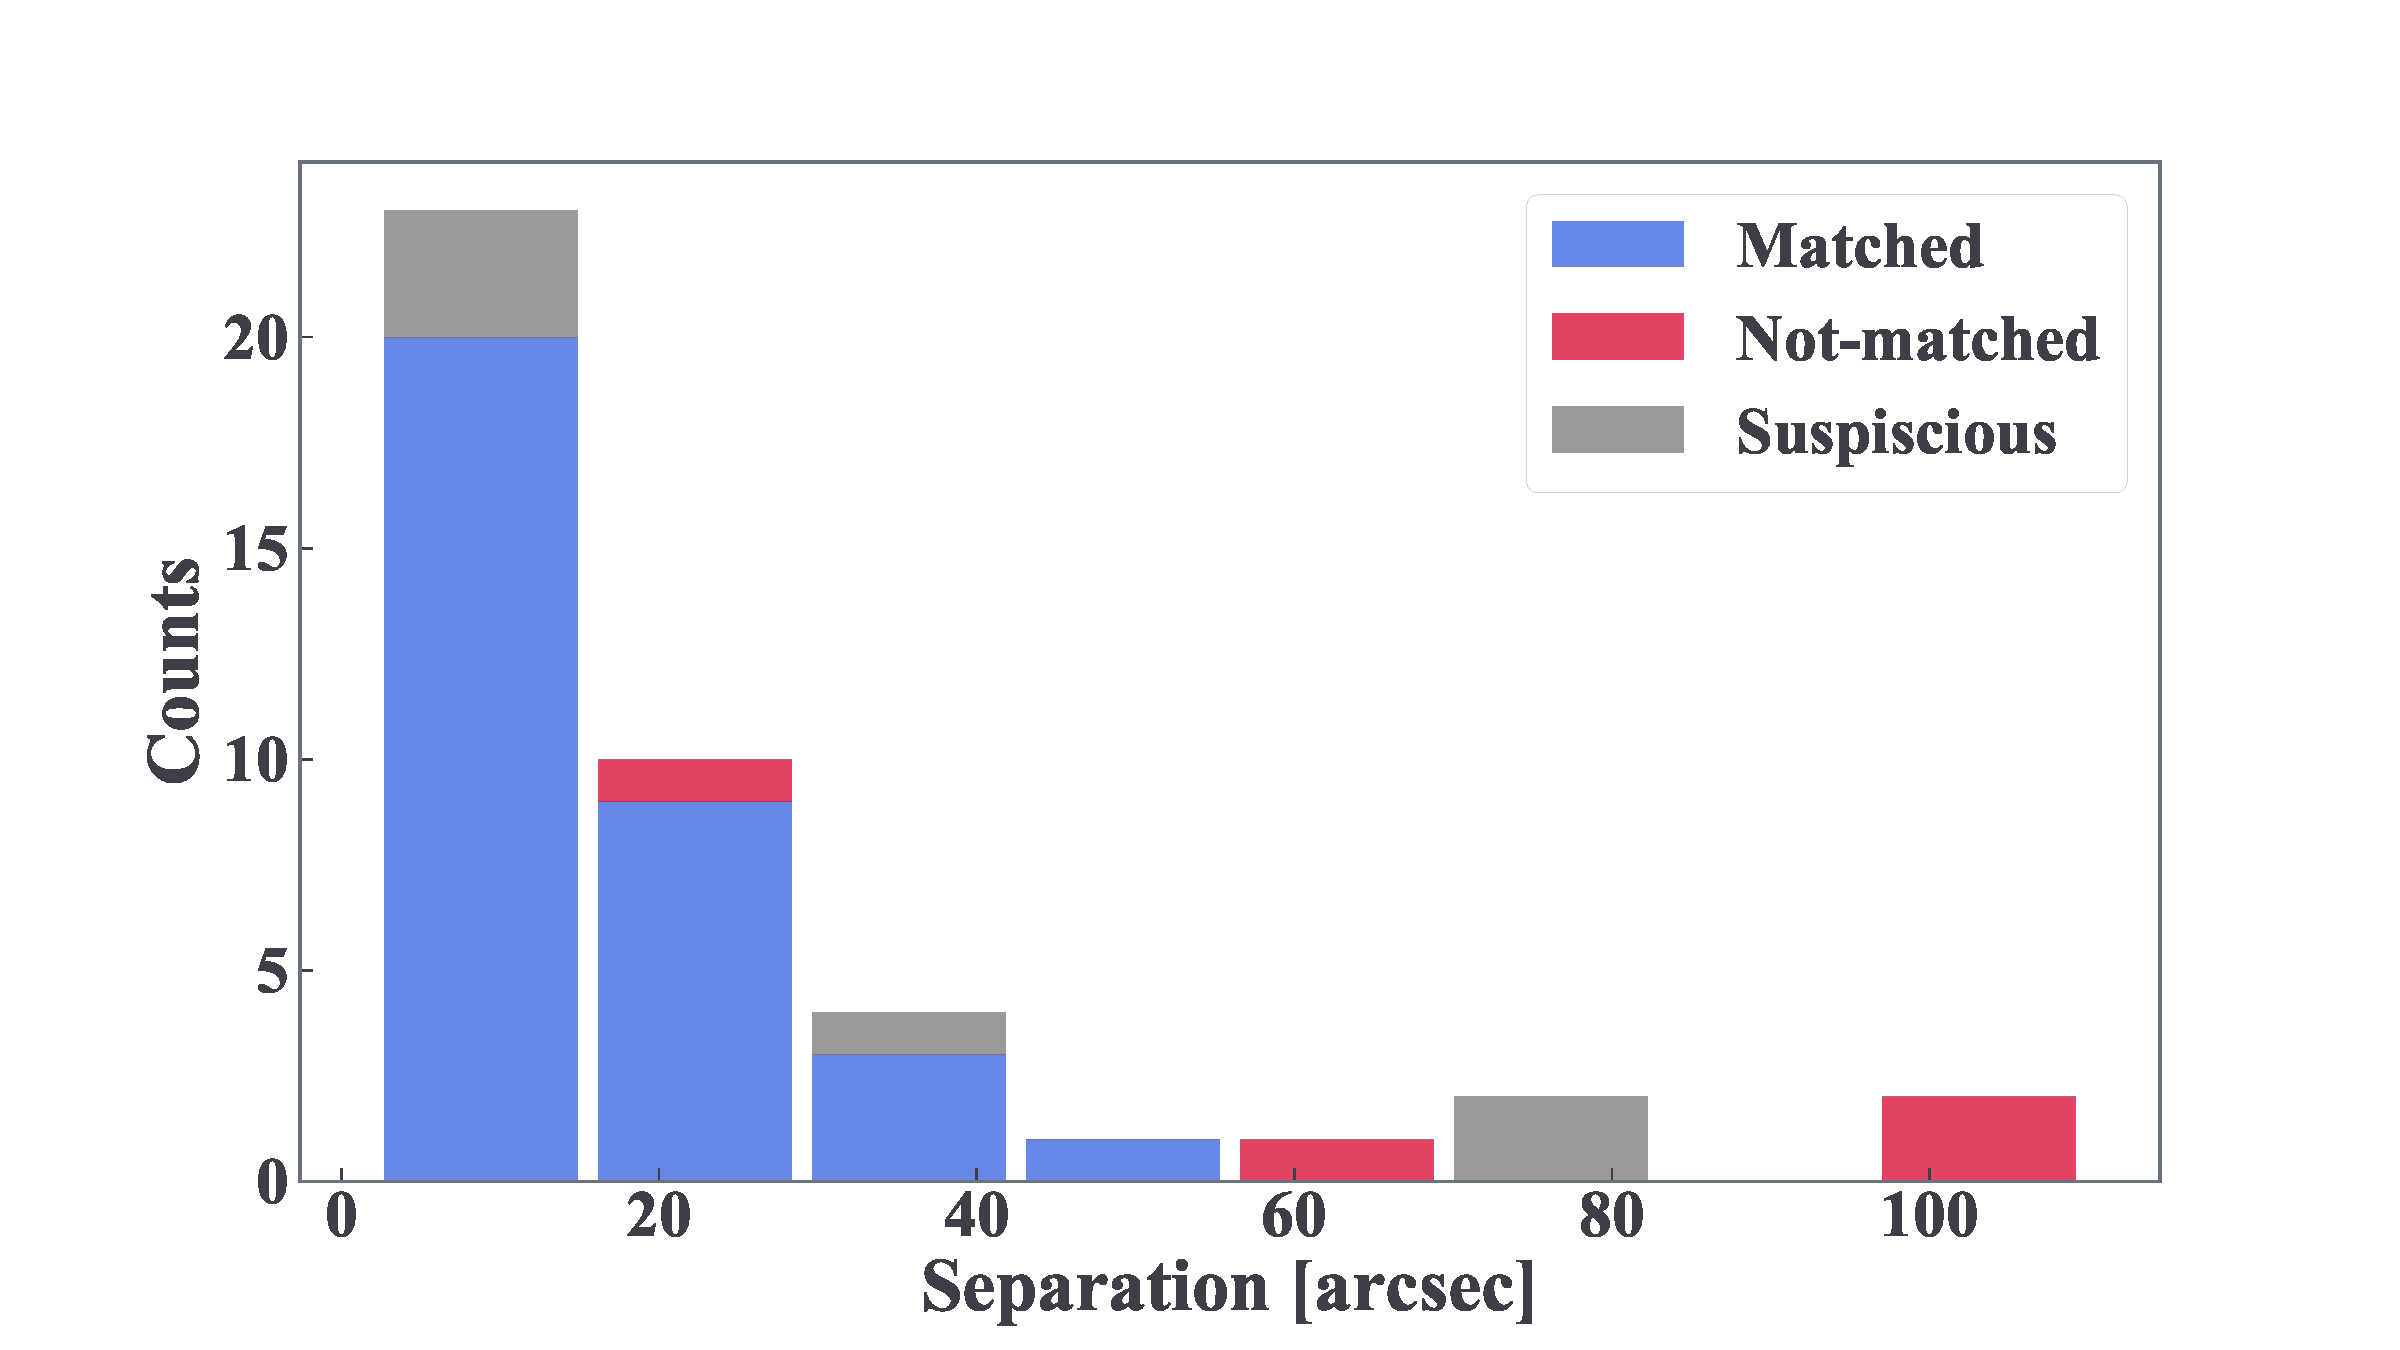
\includegraphics[width=.8\linewidth]{Chapter_4/Figures/Method_separation.pdf}
    \caption[Separation from the cross-matching]{\label{fig:separation}
        The distribution of separations of the center of radio sources from the galactic center.
        Here we put 43 galaxies and color sorted based on the result.
        The blue bar shows galaxies identified to have a radio counterpart, red one does galaxies determined not to have a counterpart, and gray for the suspicious galaxies.
        Most of the matched samples are distributed within a $40\,\mr{arcsec}$ error radius.
    }
\end{figure}

We put all galaxy images cross-matched within $120\,\mr{arcsec}$ in Appendix~\ref{chap:galaxyimages}.



\section{Select Galaxy Samples for a Reliable Analysis}\label{sec:reducegalaxysamples}

In this Section, we show some steps for selecting galaxies to do a reliable analysis.
Since we focus on the relation of galaxy radio emission with star formation activities, we should clarify the radio source and be sure that they are not originally from other sources rather than the star formation.
The radio emission arisen from the star formation activities should be proportional to the SFR in a galaxy \citep{Condon1992a, Murphy2011}.
However, elliptical galaxies have a stronger radio emission against their star formation.
In this case their radio emission would be emitted by not star-forming sources.
These radio sources are considered as Active Galactic Nuclei (AGN), which emits the radiation in a wide range of frequency due to the baryon accretion into the supermassive black hole at the center of galaxies irrelevant to the star formation \citep[e.g.,][]{Urry1995, Padovani2017}.
According to the morphology of galaxies \citep{Cortese2012}, we identify four elliptical galaxies (HRS49, 138, 178, 241) and they are not used for further calculation and discussion.
%With these operations, we finally find that there are 37 HRS galaxies are available for further analysis.

After this galaxy selection, we obtain 29 galaxies with a reliable radio counterpart arisen from the star formation activity.

As a next step, we evaluate the signal to noise ratio (SNR) of radio emission at each MWA band.
For reducing the uncertainty caused by observational errors, we assess the peak flux at each narrow band by comparing it to the local noise level and adopt flux values whose SNR is higher than five.
This analysis results in a total of 11 galaxies have no radio fluxes whose SNR is higher than the criterion.
The reason why these radio sources are detected although they do not have any fluxes with higher SNR, is \citet{Hurley-Walker2017a} determine the detection based on the SNR in the stacking images ($170\mbox{--}231\MHz$).
%\vspace{0.3cm}\\

Finally, after the cross-matching and these procedures, we confirm 18 HRS galaxies are the samples available for further analysis.
The overview of 18 samples is tabled in Appendix~\ref{chap:galaxysamples}.

%\bibliographystyle{mnras}
%%\bibliography{example} % if your bibtex file is called example.bib
%\bibliography{masterthesis}
